\documentclass[10pt]{beamer}
\usetheme{Warsaw}
\usepackage[T1]{fontenc}
\usepackage[utf8]{inputenc}
\usepackage{chronosys}
\usepackage{graphicx}
\title{Kinetic}
\author{Team member: \newline\newline Demuth Axel \newline Geraldes Pereira Dorian \newline\newline Supervisor :  \newline\newline Pierre Alliez \newline Vincent Chabannes}
\date{}
\begin{document}
\frame{\titlepage}
\begin{frame}
    \tableofcontents
\end{frame}
\section{Introduction}


\begin{frame}[plain]{objectives}
    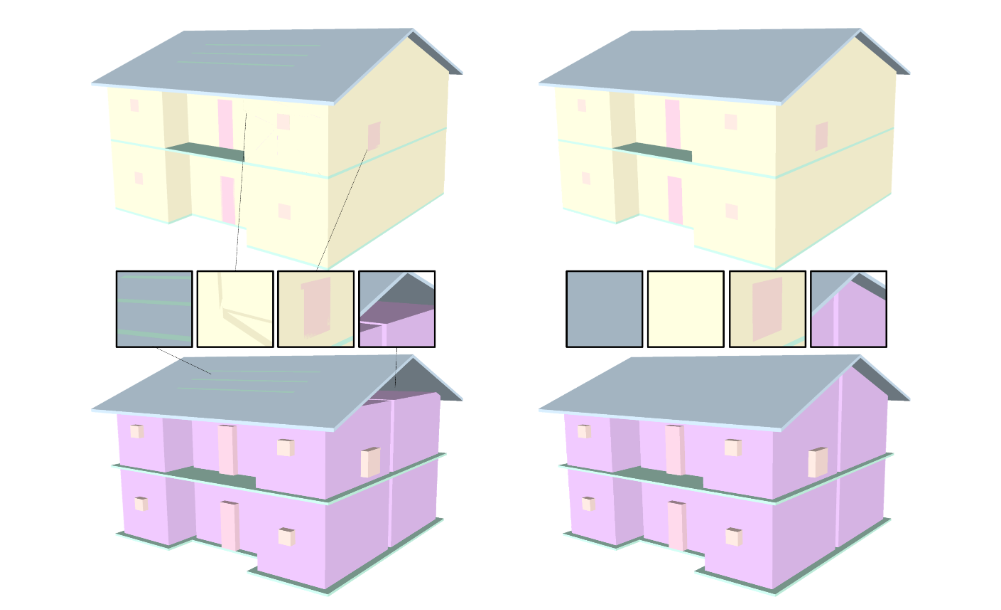
\includegraphics[scale = 0.45]{../../images/example_algorithm.png}
\end{frame}

\begin{frame}[plain]{watertight building model}
    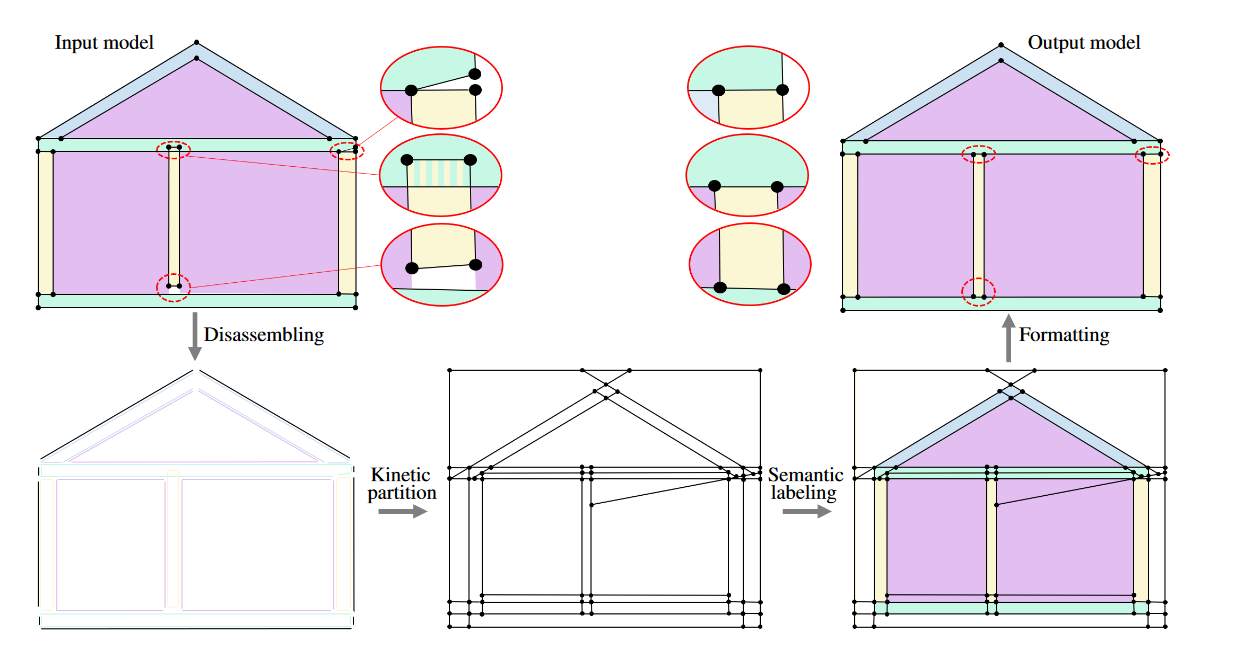
\includegraphics[scale = 0.37]{../../images/example_algorithm_2.png}
\end{frame}
\begin{frame}[plain]{watertight urban model}
    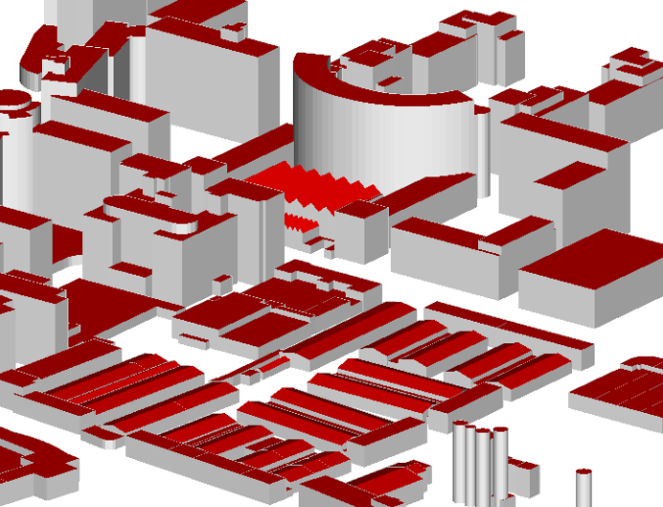
\includegraphics[scale = 0.60]{../../images/example_algorithm_3.png}
\end{frame}

\section{Tools}
\begin{frame}{Tools}
    
    
\includegraphics[scale = 0.2]{../../images/CGAL_logo.png}
    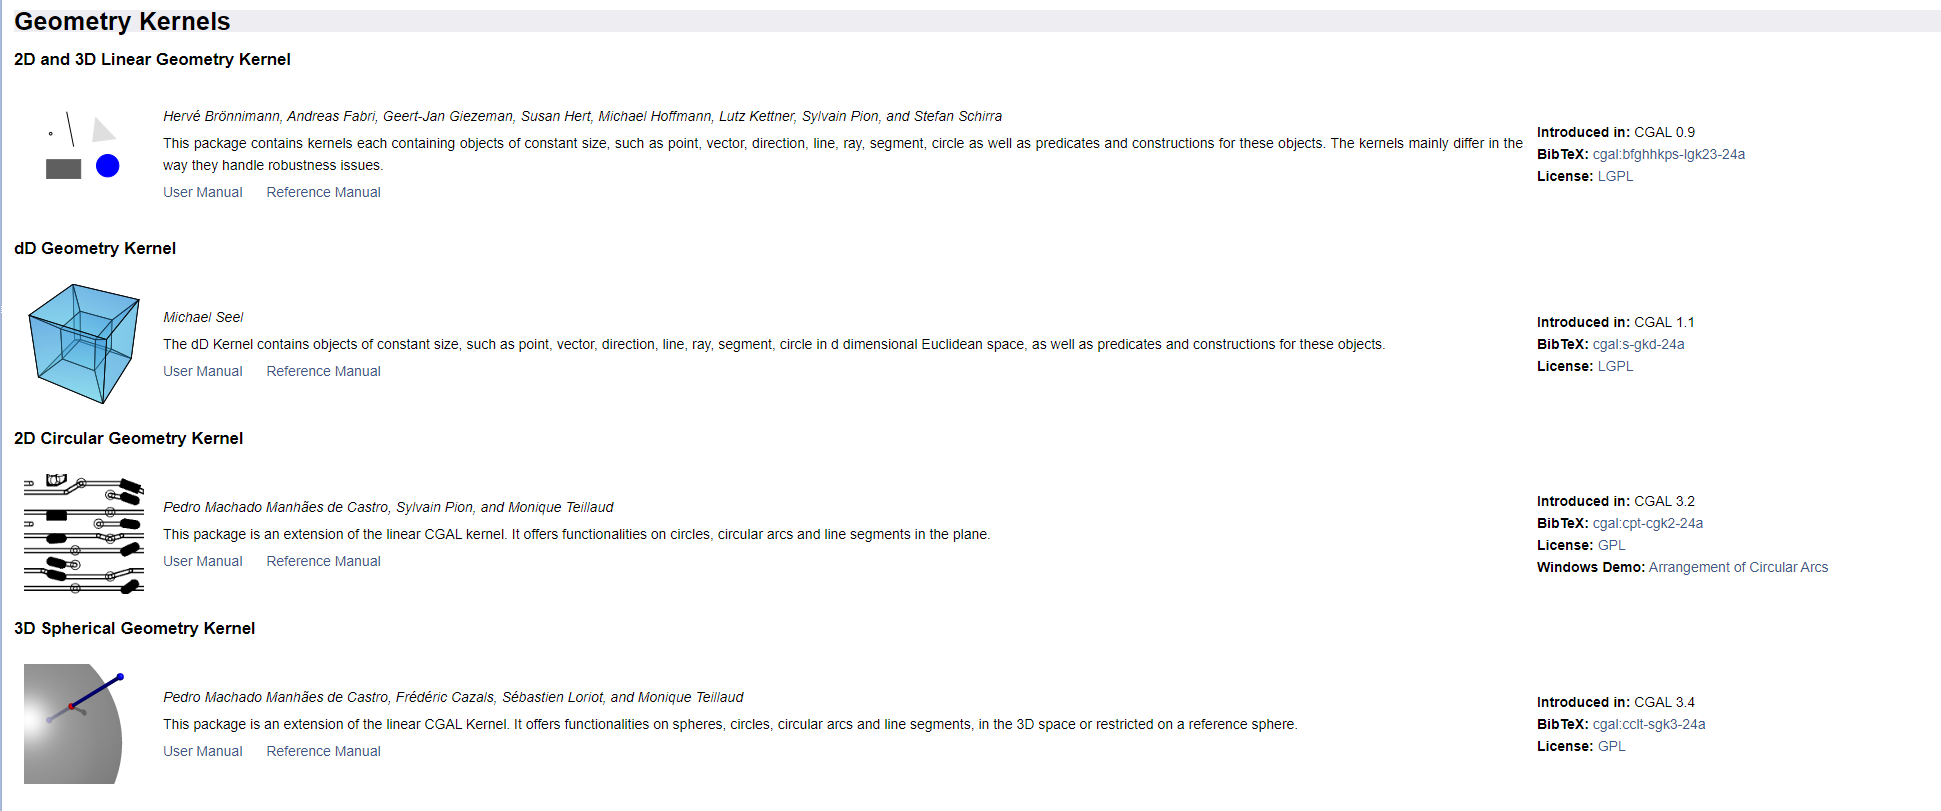
\includegraphics[scale =   0.3 ]{../../images/exemple.png}

\end{frame}



\begin{frame}[plain]{Tools}
    \begin{itemize}
        \item learn how to use CGAL package
        \item learn how to read structure mesh to use it in CGAL code
        \item learn how to use KINETIC package to fill the structure mesh  
    \end{itemize}
\end{frame}
<<<<<<< HEAD
\section{roadmap}

\begin{frame}
    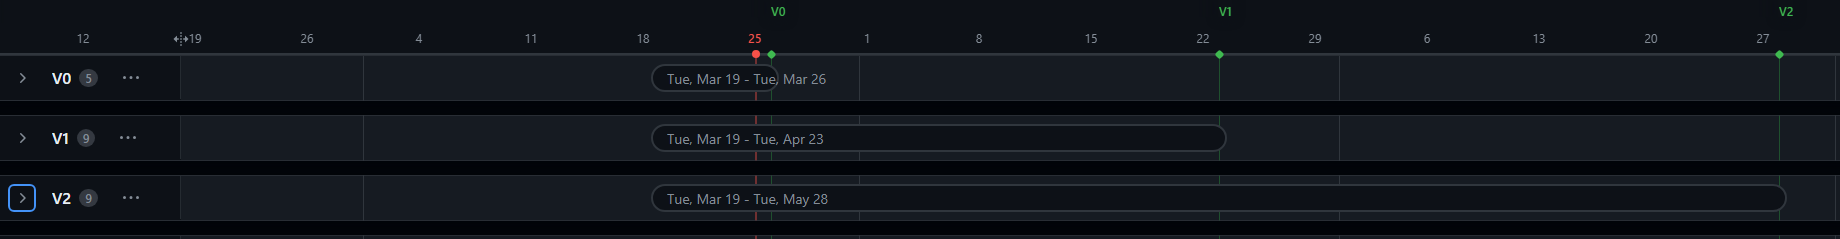
\includegraphics[scale = 0.5]{../../images/roadmap.png}
=======
\begin{frame}{reference}
    \nocite{*}
    \bibliographystyle{unsrt}
    \bibliography{../../bibliography/v0/report_bib}
>>>>>>> 13b29dd1e2ee2102972096a6c8fd76abafbc5d06
\end{frame}

\end{document}